\subsection{Environment Mapping}
In order for the aircraft to safely navigate while searching for Joe, it must first understand the environment it is moving in. State-of-the-art autonomous vehicles commonly use Red-Green-Blue-Depth cameras \cite{ref:rgbd}, allowing them to collect both visual and depth/distance information simultaneously, such as the image shown in Figure \ref{fig:rgbd}. While these cameras are powerful, they are also expensive, with the cheapest unit found to cost almost \$5000 \cite{ref:rgbdcost}. Instead, a low-cost approach was chosen that combines data from the camera and LiDAR shown in Section \ref{sec:sensing} in order to approximate the capability of an RGB-D camera.\\

\begin{figure}[!ht]
	\centering
	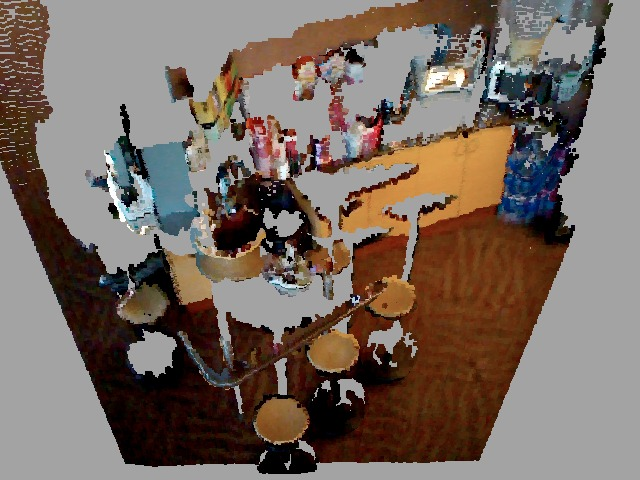
\includegraphics[width=200pt]{\IMAGEPATH /Data/rgbd}
	\caption{An example of RGB-Depth data}
	\label{fig:rgbd}
\end{figure}

Mapping is initiated once the aircraft begins maneuver M3, as described in Section \ref{sec:flightmaneuvers}. During this maneuver, the LiDAR will scan the area in front of the aircraft, ranging from $\pm$85$^\circ$ in the horizontal direction, in 5$^\circ$ increments, and from 20$^\circ$ below to 90$^\circ$ above the aircraft, in 1.25$^\circ$ increments. At each increment, the LiDAR will calculate the distance to the nearest object in space.\\

Rather than store each of these distance measurements as points in space, the data is stored in the form of an occupancy grid. The world around the aircraft is discretised into 10cm cells (or voxels), and when the LiDAR detects an object at a point in space, the corresponding voxel in the grid is then ``filled''; this approach will make real-time path planning and obstacle avoidance algorithms computationally feasible on the Raspberry Pi by reducing the volume of data to be processed.\\

Figure \ref{fig:scan} shows the progression of data acquisition using the LiDAR. When the aircraft first enters maneuver M3, the occupancy grid is initially empty, as no data has been acquired (Figure \ref{fig:scaninit}). The occupancy grid is gradually filled as the LiDAR performs its sweep, with Figures \ref{fig:scanten} and \ref{fig:scanminute} showing 10s and 60s of data acquisition respectively. This data will then be filtered (to remove isolated voxels) and clustered (to generate larger ``obstacles'') in order to generate a safe flight path.

\begin{figure}[!ht]
	\centering
	\begin{subfigure}[b]{0.50\textwidth}
		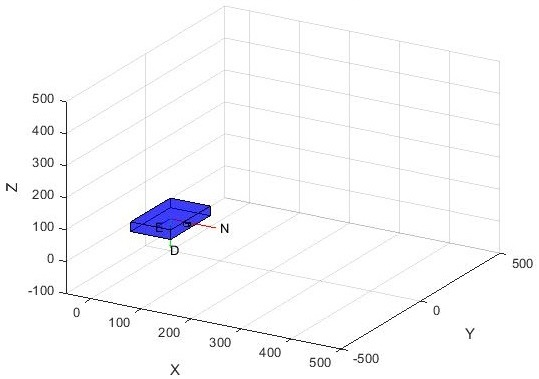
\includegraphics[width=\textwidth]{\IMAGEPATH Data/voxelize0s}
		\caption{Initial (empty) environment}
		\label{fig:scaninit}
	\end{subfigure}
	
	\begin{subfigure}[b]{0.50\textwidth}
		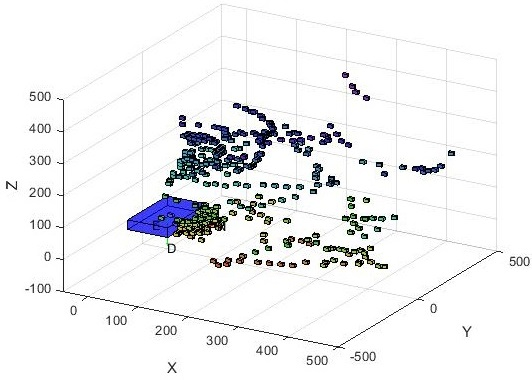
\includegraphics[width=\textwidth]{\IMAGEPATH Data/voxelize10s}
		\caption{10s of data acquisition}
		\label{fig:scanten}
	\end{subfigure}
	
	\begin{subfigure}[b]{0.50\textwidth}
		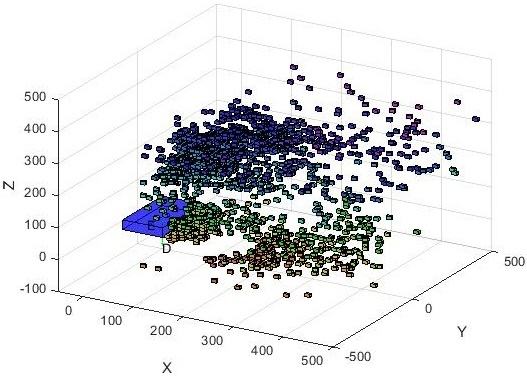
\includegraphics[width=\textwidth]{\IMAGEPATH Data/voxelize60s}
		\caption{60s of data acquisition}
		\label{fig:scanminute}
	\end{subfigure}
	\caption{Scanning the environment with the LiDAR; data is coloured according to height above ground}
	\label{fig:scan}
\end{figure}